\subsubsection*{Exercise 0.3.7. (Gapry)}

\begin{flushleft}

\textbf{Part B} \\
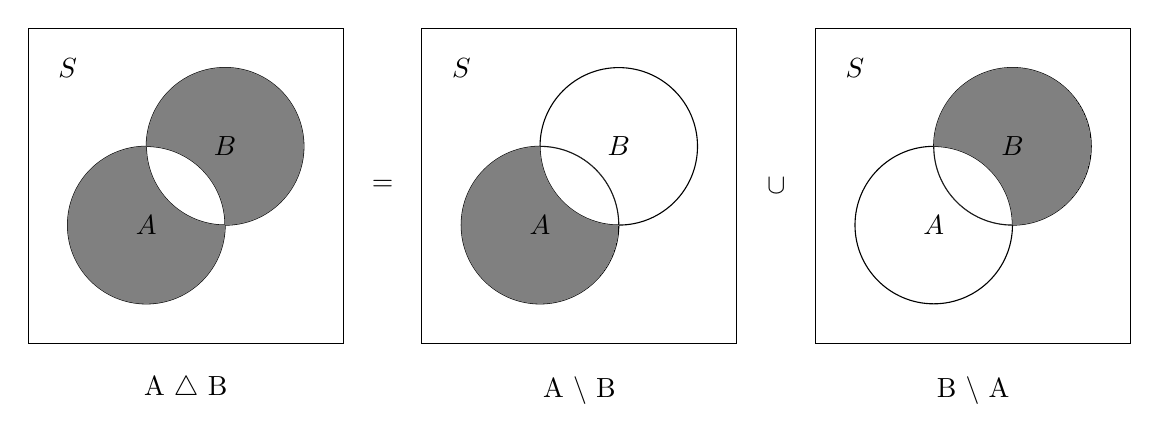
\begin{tikzpicture}
    \begin{scope}[shift={(-6, 0)}]
        \def\firstcircle  {(-0.5, -0.5) circle(1)}
        \def\secondcircle {( 0.5,  0.5) circle(1)}
        
        \draw (-2,-2) rectangle (2, 2);  % Draw the universe set S
        \draw \firstcircle;              % Draw subset A
        \draw \secondcircle;             % Draw subset B

        \fill[even odd rule, gray] \firstcircle \secondcircle;
        
        \node at (-1.5,  1.5) {$S$};  % Label the universe set 
        \node at (-0.5, -0.5) {$A$};  % Label subset A
        \node at ( 0.5,  0.5) {$B$};  % Label subset A
        
        \node[below] at (0, -2.3) {A $\triangle$ B};
    \end{scope}

    \node at (-3.5,0) {$=$};

    % Figure 2: Venn diagram of A \ B
    \begin{scope}[shift={(-1, 0)}]
        \def\firstcircle  {(-0.5, -0.5) circle(1)}
        \def\secondcircle {( 0.5,  0.5) circle(1)}
    
        \draw (-2,-2) rectangle (2, 2);  % Draw the universe set S
        \draw \firstcircle;              % Draw subset A
        \draw \secondcircle;             % Draw subset B
        
        \begin{scope}
            \clip \firstcircle ;
            \fill[gray,even odd rule] \firstcircle \secondcircle;
        \end{scope}
        
        \node at (-1.5,  1.5) {$S$};  % Label the universe set 
        \node at (-0.5, -0.5) {$A$};  % Label subset A
        \node at ( 0.5,  0.5) {$B$};  % Label subset A
        \node[below] at (0,-2.3) {A $\setminus$ B};
    \end{scope}

    \node at (1.5,0) {$\cup$};

    % Figure 3: Venn diagram of B \ A
    \begin{scope}[shift={(4, 0)}]
        \def\firstcircle  {(-0.5, -0.5) circle(1)}
        \def\secondcircle {( 0.5,  0.5) circle(1)}
    
        \draw (-2,-2) rectangle (2, 2);  % Draw the universe set S
        \draw \firstcircle;              % Draw subset A
        \draw \secondcircle;             % Draw subset B
        
        \begin{scope}
            \clip \secondcircle;
            \fill[gray,even odd rule] \secondcircle \firstcircle;
        \end{scope}
        
        \node at (-1.5,  1.5) {$S$};  % Label the universe set 
        \node at (-0.5, -0.5) {$A$};  % Label subset A
        \node at ( 0.5,  0.5) {$B$};  % Label subset A
        \node[below] at (0, -2.3) {B $\setminus$ A};
    \end{scope}
\end{tikzpicture}

\textbf{Part C} \\
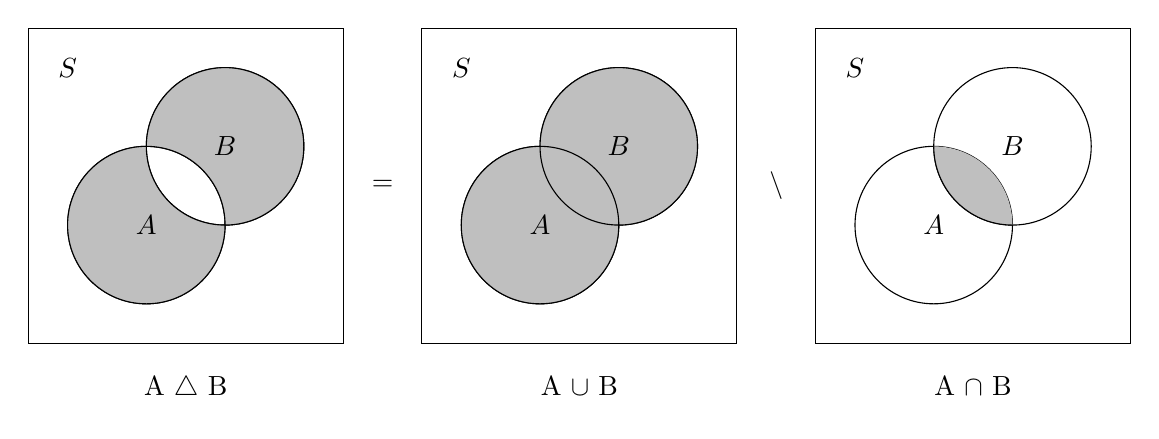
\begin{tikzpicture}
    \begin{scope}[shift={(-6, 0)}]
        \def\firstcircle  {(-0.5, -0.5) circle(1)}
        \def\secondcircle {( 0.5,  0.5) circle(1)}
        
        \draw (-2,-2) rectangle (2, 2);  % Draw the universe set S
        \draw \firstcircle;              % Draw subset A
        \draw \secondcircle;             % Draw subset B

        \fill[even odd rule, draw = black, fill = lightgray] \firstcircle \secondcircle;
        
        \node at (-1.5,  1.5) {$S$};  % Label the universe set 
        \node at (-0.5, -0.5) {$A$};  % Label subset A
        \node at ( 0.5,  0.5) {$B$};  % Label subset A
        
        \node[below] at (0, -2.3) {A $\triangle$ B};
    \end{scope}

    \node at (-3.5,0) {$=$};

    % Figure 2: Venn diagram of A union B
    \begin{scope}[shift={(-1, 0)}]
        \def\firstcircle  {(-0.5, -0.5) circle(1)}
        \def\secondcircle {( 0.5,  0.5) circle(1)}
    
        \draw (-2,-2) rectangle (2, 2);  % Draw the universe set S
        \draw \firstcircle;              % Draw subset A
        \draw \secondcircle;             % Draw subset B
        
        \begin{scope}
            \filldraw[draw = black, fill = lightgray] \firstcircle \secondcircle;
        \end{scope}
        
        \node at (-1.5,  1.5) {$S$};  % Label the universe set 
        \node at (-0.5, -0.5) {$A$};  % Label subset A
        \node at ( 0.5,  0.5) {$B$};  % Label subset A
        \node[below] at (0, -2.3) {A $\cup $ B};
    \end{scope}

    \node at (1.5,0) {$\setminus$};

    % Figure 3: Venn diagram of A intersection B
    \begin{scope}[shift={(4, 0)}]
        \def\firstcircle  {(-0.5, -0.5) circle(1)}
        \def\secondcircle {( 0.5,  0.5) circle(1)}
    
        \draw (-2,-2) rectangle (2, 2);  % Draw the universe set S
        \draw \firstcircle;              % Draw subset A
        \draw \secondcircle;             % Draw subset B
        
        \begin{scope}
            \clip \firstcircle ;
            \fill[draw = black, fill = lightgray] \secondcircle;
        \end{scope}
        
        \node at (-1.5,  1.5) {$S$};  % Label the universe set 
        \node at (-0.5, -0.5) {$A$};  % Label subset A
        \node at ( 0.5,  0.5) {$B$};  % Label subset A
        \node[below] at (0, -2.3) {A $\cap$ B};
    \end{scope}
\end{tikzpicture}

\end{flushleft}